\section{Portfolio Optimization Results}\label{sec:allocation}
\begin{correction}

We compare six allocation strategies from November 2019 to November 2025. Two minimize variance or CVaR using historical returns. Two use scenarios simulated from the ARMA-EGARCH R-vine. We also include the equally weighted portfolio (1/N) and a minimum-CVaR strategy that uses the same ARMA-EGARCH margins with a Gaussian copula. Short selling is prohibited, asset weights are capped at 50\%, and the risk-free rate is set to 2\%.

\subsection{Backtest Design}

Portfolios are rebalanced every five trading sessions, for 302 rebalances between November 4, 2019 and November 3, 2025. At each rebalance, \texttt{rugarch} estimates the ARMA-EGARCH margins with standardized Student-t innovations using up to 1,000 prior daily returns. The copula is fitted to the last 504 pseudo-observations. We simulate next-day returns as
\[
r_{i,t+1} = \hat\mu_{i,t+1} + \hat\sigma_{i,t+1}\,(F^{\mathrm{std}}_{\nu_i})^{-1}(U_i),
\]
where \(U_i\) is the simulated uniform component for asset \(i\).

We use 10,000 scenarios per draw and five random seeds for the simulated CVaR strategies. The simulated minimum-variance strategy uses the first draw. We minimize 95\% CVaR using the formulation of \citet{rockafellar2000}. The historical strategies use the most recent 252 observed returns. Transaction costs are 10 basis points per unit of turnover, and weights drift with prices between rebalances.

\subsection{Strategy Performance}

\begin{table}[H]
\centering
\resizebox{\textwidth}{!}{%
\begin{tabular}{lrrrrrrrrr}
\toprule
Strategy & Total return & Ann. return & Ann. vol. & Sharpe & Sortino & Max DD & Calmar & Daily CVaR & Turnover \\
 & (\%) & (\%) & (\%) & & & (\%) & & 95\% (\%) & /year \\
\midrule
Equal weight (1/N) & 278.09 & 24.89 & 19.25 & 1.189 & 1.705 & -34.70 & 0.717 & 2.68 & 1.4 \\
Historical MinVar & 55.73 & 7.68 & 8.61 & 0.660 & 0.920 & -16.66 & 0.461 & 1.23 & 0.8 \\
Historical MinCVaR & 54.59 & 7.55 & 8.66 & 0.641 & 0.891 & -17.04 & 0.443 & 1.24 & 1.1 \\
MinVar R-vine ARMA-EGARCH & 65.90 & 8.83 & 8.19 & 0.834 & 1.172 & -15.62 & 0.565 & 1.16 & 6.3 \\
MinCVaR R-vine ARMA-EGARCH & 66.95 & 8.94 & 8.23 & 0.844 & 1.185 & -15.74 & 0.568 & 1.16 & 6.2 \\
Gaussian copula MinCVaR & 66.13 & 8.85 & 8.13 & 0.843 & 1.188 & -15.60 & 0.568 & 1.15 & 5.9 \\
\bottomrule
\end{tabular}}
\caption{Out-of-sample strategy performance, net of transaction costs}
\label{tab:perf}
\end{table}

The ARMA-EGARCH R-vine CVaR strategy earns a total return of 66.95\%, compared with 55.73\% for historical minimum variance. Their Sharpe ratios are 0.844 and 0.660, respectively. With the same margins, Gaussian copula CVaR achieves a Sharpe ratio of 0.843. The equally weighted portfolio earns 278.09\% in total and records a maximum drawdown of $-34.70\%$.

\subsection{Performance and Portfolio Weights Over Time}

Figure~\ref{fig:relative} shows cumulative wealth relative to the historical minimum-variance benchmark. From February 20 to March 23, 2020, the ARMA-EGARCH R-vine CVaR strategy returns $-8.83\%$, compared with $-9.62\%$ for historical minimum variance and $-7.82\%$ for Gaussian copula CVaR.

\begin{figure}[H]
\centering
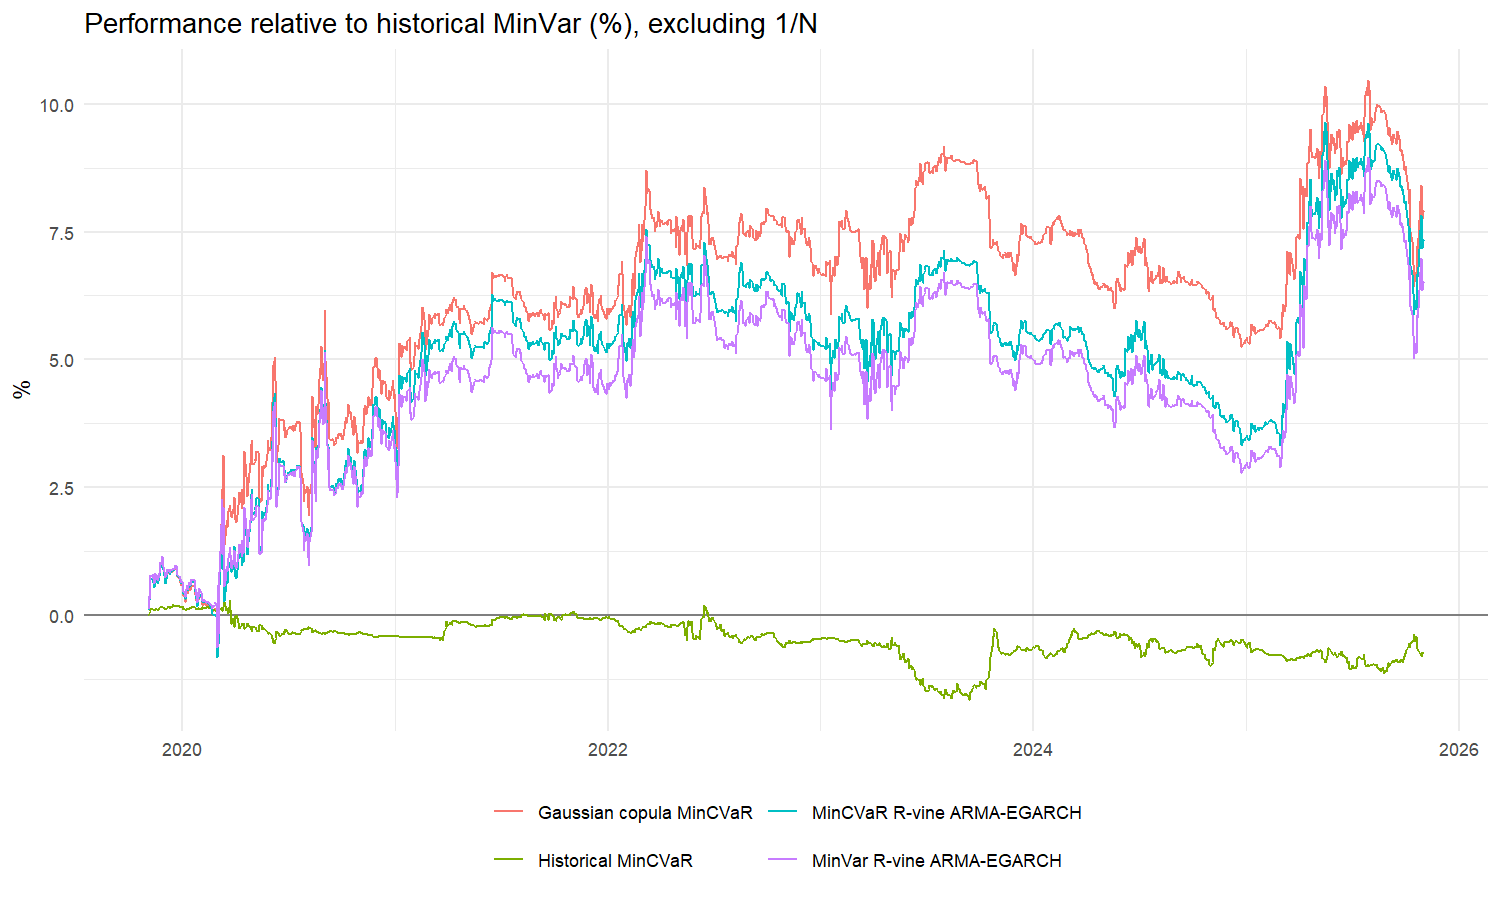
\includegraphics[width=0.95\textwidth]{figures/04_relative_performance.png}
\caption{Performance relative to historical minimum variance, excluding the equally weighted portfolio}
\label{fig:relative}
\end{figure}

Figure~\ref{fig:weights} shows the weekly weights for the first ARMA-EGARCH R-vine CVaR draw. On average, the portfolio allocates 49.9\% to BND, 28.2\% to SPY, 21.6\% to gold, and 0.3\% to Bitcoin. The small Bitcoin allocation limits the influence of its tail dependence on the portfolio.

\begin{figure}[H]
\centering
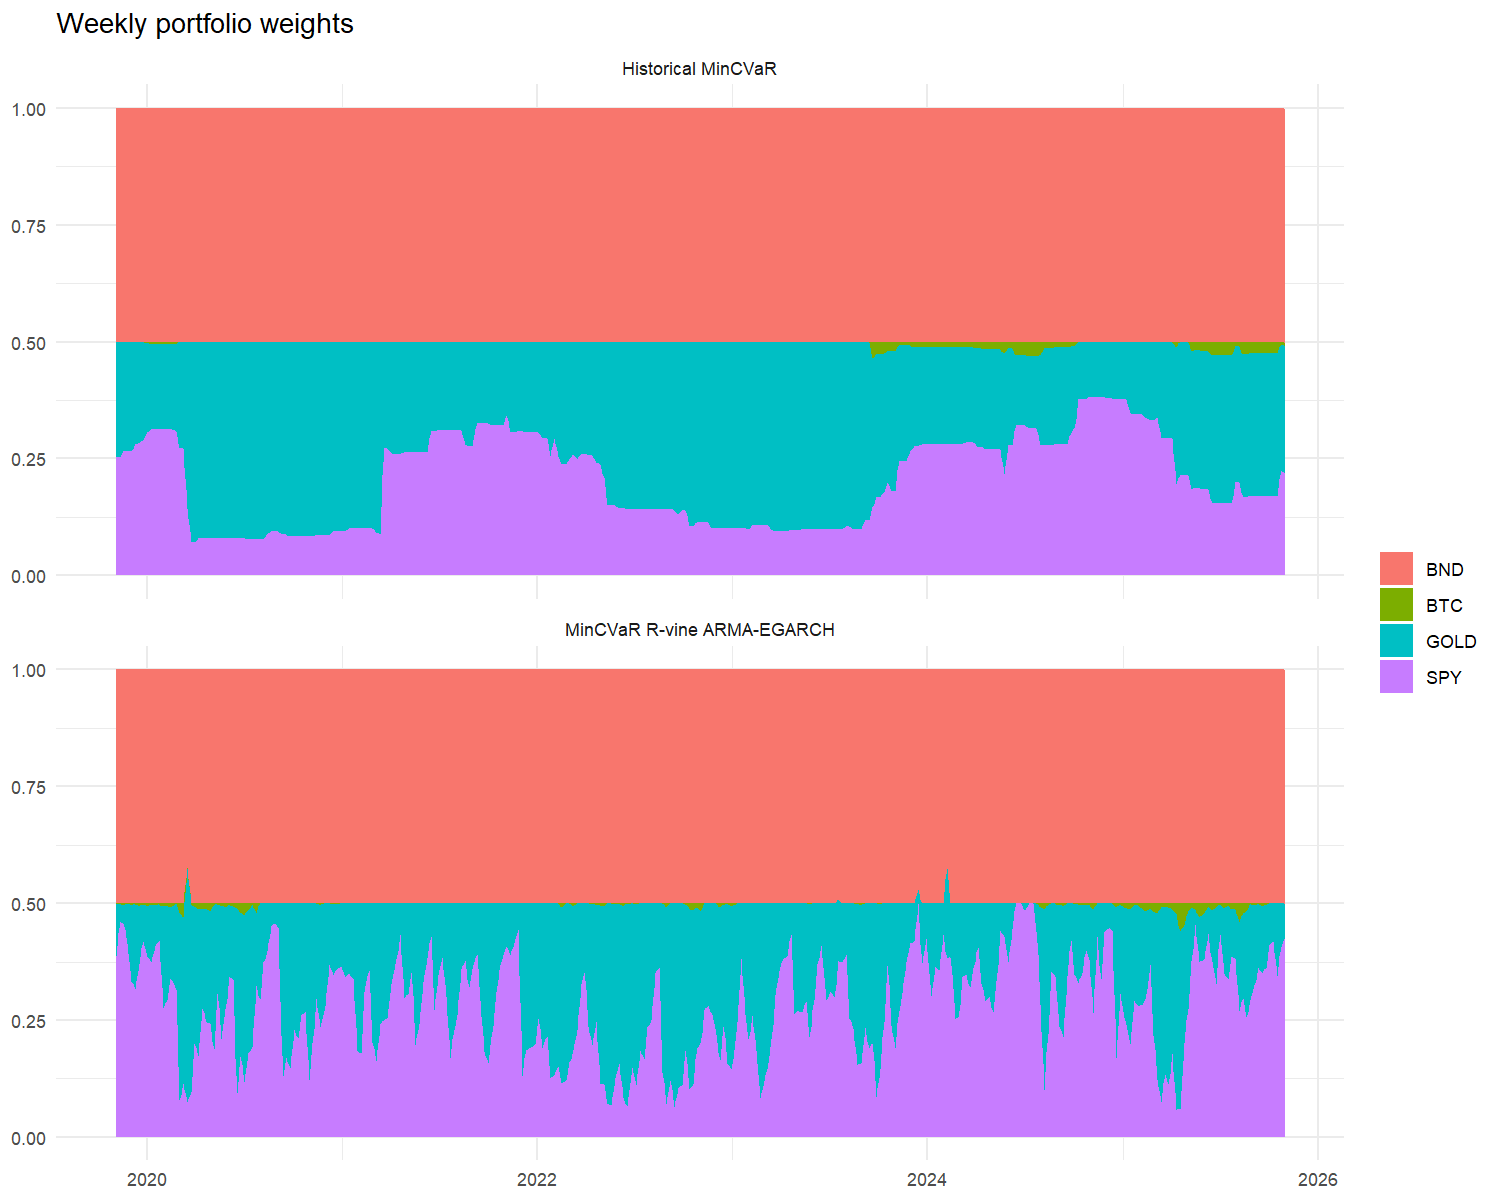
\includegraphics[width=0.95\textwidth]{figures/05_weights.png}
\caption{Weekly weights for ARMA-EGARCH R-vine CVaR and historical CVaR portfolios}
\label{fig:weights}
\end{figure}

\subsection{Statistical Significance and Monte Carlo Variation}\label{sec:monte-carlo}

We assess performance differences with a circular block bootstrap \citep{politis1992} on paired daily returns. We use 2,000 replications and blocks of 20 trading sessions. The comparisons use the first random seed.

\begin{table}[H]
\centering
\resizebox{\textwidth}{!}{%
\begin{tabular}{lrrrrrr}
\toprule
Comparison strategy & $\Delta$ Sharpe & p-value & $\Delta$ CVaR (pp) & p-value & $\Delta$ Max DD (pp) & p-value \\
\midrule
Equal weight (1/N) & -0.343 & 0.433 & -1.510 & 0.000 & 18.885 & 0.004 \\
Historical MinVar & 0.186 & 0.179 & -0.063 & 0.147 & 0.842 & 0.573 \\
Historical MinCVaR & 0.204 & 0.182 & -0.075 & 0.112 & 1.227 & 0.406 \\
MinVar R-vine ARMA-EGARCH & 0.011 & 0.564 & 0.007 & 0.222 & -0.190 & 0.402 \\
Gaussian copula MinCVaR & -0.031 & 0.386 & 0.026 & 0.093 & -0.464 & 0.441 \\
\bottomrule
\end{tabular}}
\caption{Performance differences between ARMA-EGARCH R-vine CVaR and the comparison strategies}
\end{table}

The Sharpe comparison with historical minimum variance gives a p-value of 0.179. The comparison with Gaussian copula CVaR gives a p-value of 0.386. Neither difference is statistically significant at the 5\% level.

\begin{table}[H]
\centering
\resizebox{\textwidth}{!}{%
\begin{tabular}{lrrrr}
\toprule
Strategy & Scenarios & Sharpe & Total return (\%) & Max DD (\%) \\
\midrule
MinCVaR R-vine ARMA-EGARCH & 10\,000 & 0.827 -- 0.865 & 65.78 -- 68.30 & -15.92 -- -15.51 \\
MinCVaR R-vine ARMA-EGARCH & 500 & 0.795 -- 0.937 & 62.85 -- 74.08 & -16.34 -- -15.43 \\
Gaussian copula MinCVaR & 10\,000 & 0.800 -- 0.877 & 63.25 -- 68.07 & -15.93 -- -15.27 \\
\bottomrule
\end{tabular}}
\caption{Minimum and maximum across five random seeds}
\label{tab:mc}
\end{table}

For ARMA-EGARCH R-vine CVaR, Sharpe ranges from 0.795 to 0.937 with 500 scenarios and from 0.827 to 0.865 with 10,000. The ranges show how sensitive the results are to the number of scenarios.

\subsection{Value at Risk and Expected Shortfall Backtests}

For the equally weighted portfolio, we forecast 95\% and 99\% VaR and 97.5\% Expected Shortfall over 1,508 trading sessions. Model parameters are re-estimated weekly, and conditional volatility is updated daily. We use the VaR tests of \citet{kupiec1995} and \citet{christoffersen1998} and the ES test of \citet{mcneil2000}.

\begin{table}[H]
\centering
\resizebox{\textwidth}{!}{%
\begin{tabular}{lrrrrrrr}
\toprule
Model & Exceed. & Kupiec p & Christ. p & Exceed. & Kupiec p & Christ. p & ES p \\
 & VaR 95\% & 95\% & 95\% & VaR 99\% & 99\% & 99\% & 97.5\% \\
\midrule
R-vine ARMA-EGARCH & 4.78 & 0.686 & 0.878 & 1.06 & 0.814 & 0.819 & 0.333 \\
EGARCH + Gaussian copula & 4.78 & 0.686 & 0.878 & 1.06 & 0.814 & 0.819 & 0.264 \\
EGARCH + independence & 6.50 & 0.011 & 0.021 & 1.26 & 0.329 & 0.488 & 0.692 \\
Historical simulation (252 days) & 4.58 & 0.443 & 0.665 & 1.33 & 0.225 & 0.366 & 0.168 \\
Normal variance-covariance (252 days) & 4.04 & 0.079 & 0.137 & 1.33 & 0.225 & 0.366 & 0.022 \\
\bottomrule
\end{tabular}}
\caption{VaR and ES backtests for the equally weighted portfolio}
\label{tab:var}
\end{table}

The ARMA-EGARCH R-vine and Gaussian copula models both record exceedance rates of 4.78\% and 1.06\%, compared with expected rates of 5\% and 1\%. With independence, the 95\% VaR exceedance rate rises to 6.50\% (Kupiec p-value 0.011). The ES test gives p-values of 0.333 for the R-vine and 0.264 for the Gaussian copula. At the 5\% level, the VaR coverage and ES tests do not reject either model.

\begin{figure}[H]
\centering
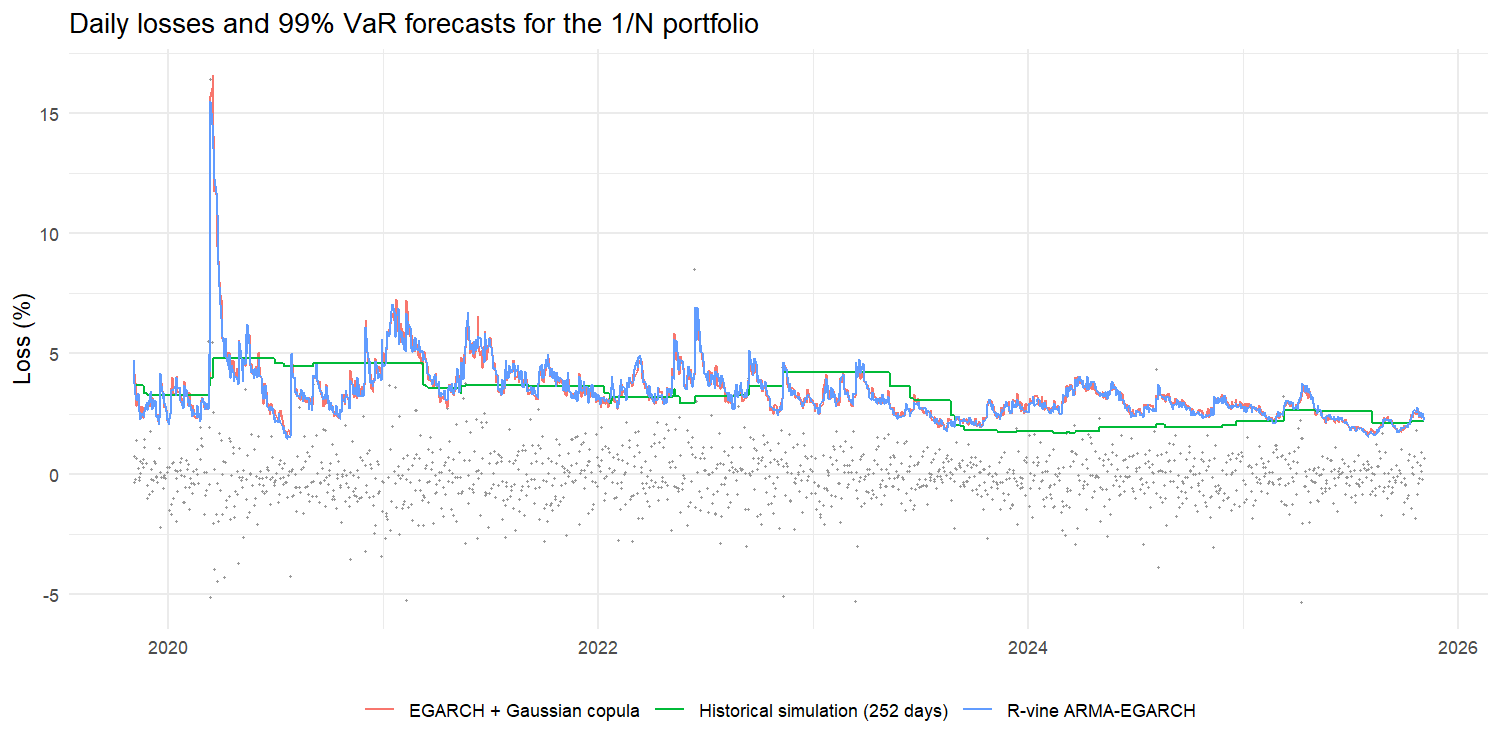
\includegraphics[width=0.95\textwidth]{figures/06_var99.png}
\caption{Daily losses and 99\% VaR forecasts for the equally weighted portfolio}
\end{figure}

\subsection{Practical Implications}

The ARMA-EGARCH R-vine CVaR strategy turns over 6.2 times the portfolio per year, compared with 0.8 for historical minimum variance. This difference matters when interpreting net performance. The similar results for the two copulas with identical margins should also be read in light of the observed weights, especially the small Bitcoin allocation.
\end{correction}

\section{Conclusion}

This study combines ARMA-GARCH models and vine copulas to quantify extreme dependence among US equities, Bitcoin, bonds, and gold from 2016 to 2025. The estimates identify a shift in the relationships among these assets and illustrate the limits of linear correlations for describing joint extremes during crises. Three findings stand out.

\begin{enumerate}
  \item Bitcoin shifts from near independence with gold and equities before 2020 to a closer relationship with equities afterward. Kendall's $\tau$ with SPY is 0.24 in the post-COVID period and around 0.25 in 2025, while lower-tail dependence is moderate (0.09 during the crisis and 0.12 afterward). The BND--SPY relationship shifts from negative before COVID ($\tau=-0.14$, LTD = 0.01) to positive afterward ($\tau=0.14$, UTD = LTD = 0.12), consistent with weaker bond hedging. In 2022, the minimum-risk strategies lose around 10\% as equities and bonds fall together. Gold and bonds remain positively dependent, with weaker tail dependence after 2022.
  \item The standardized Student-t distribution is used both to transform standardized residuals to uniforms and to simulate returns for risk measurement.
  \item The ARMA-EGARCH R-vine CVaR strategy achieves a Sharpe ratio of 0.844, versus 0.660 for historical minimum variance. With the same margins and a Gaussian copula, the Sharpe ratio is 0.843. The comparison between the two CVaR strategies gives a p-value of 0.386. The low weight of Bitcoin in minimum-risk portfolios limits the influence of its tail dependence.
\end{enumerate}

The framework extends conventional correlation-based analysis to multi-asset portfolios that include crypto-assets.

These results motivate further work on the use of tail dependence in allocation decisions.

Future work could examine how transaction costs affect the choice of recalibration frequency, broaden the asset universe, and develop conditional vine copulas with macroeconomic variables such as expected inflation, real rates, and the VIX. The latter extension would test whether the model can anticipate changes in dependence before episodes of stress.
Another extension would test portfolios with a material Bitcoin allocation, for example through a minimum-weight constraint or a return target, where asymmetric dependence may have a greater effect on the allocation.

% =====================================================================================================
\begin{correction}
\begin{thebibliography}{99}
\bibitem[Aas et~al.(2009)]{aas2009} Aas, K., Czado, C., Frigessi, A. and Bakken, H. (2009). ``Pair-copula constructions of multiple dependence''. In: \emph{Insurance: Mathematics and Economics} 44.2, pp.~182--198.
\bibitem[Bedford and Cooke(2002)]{bedford2002} Bedford, T. and Cooke, R. M. (2002). ``Vines -- a new graphical model for dependent random variables''. In: \emph{The Annals of Statistics} 30.4, pp.~1031--1068.
\bibitem[Christoffersen(1998)]{christoffersen1998} Christoffersen, P. F. (1998). ``Evaluating interval forecasts''. In: \emph{International Economic Review} 39.4, pp.~841--862.
\bibitem[Dissmann et~al.(2013)]{dissmann2013} Dissmann, J., Brechmann, E. C., Czado, C. and Kurowicka, D. (2013). ``Selecting and estimating regular vine copulae and application to financial returns''. In: \emph{Computational Statistics \& Data Analysis} 59, pp.~52--69.
\bibitem[Evkaya et~al.(2024)]{evkaya2024} Evkaya, O. et al. (2024). ``Vine copula approach to understand the financial dependence of the Istanbul stock exchange index''. In: \emph{Computational Economics} 64.5, pp.~2935--2980.
\bibitem[Ghalanos(n.d.)]{rugarch} Ghalanos, A. \emph{rugarch: Univariate GARCH models}. R package.
\bibitem[Kupiec(1995)]{kupiec1995} Kupiec, P. H. (1995). ``Techniques for verifying the accuracy of risk measurement models''. In: \emph{The Journal of Derivatives} 3.2, pp.~73--84.
\bibitem[McNeil and Frey(2000)]{mcneil2000} McNeil, A. J. and Frey, R. (2000). ``Estimate of tail-related risk measures for heteroscedastic financial time series: an extreme value approach''. In: \emph{Journal of Empirical Finance} 7.3--4, pp.~271--300.
\bibitem[Nelson(1991)]{nelson1991} Nelson, D. B. (1991). ``Conditional heteroskedasticity in asset returns: A new approach''. In: \emph{Econometrica} 59.2, pp.~347--370.
\bibitem[Politis and Romano(1992)]{politis1992} Politis, D. N. and Romano, J. P. (1992). ``A circular block-resampling procedure for stationary data''. In: LePage, R. and Billard, L. (eds.), \emph{Exploring the Limits of Bootstrap}. Wiley, pp.~263--270.
\bibitem[Rockafellar and Uryasev(2000)]{rockafellar2000} Rockafellar, R. T. and Uryasev, S. (2000). ``Optimization of conditional value-at-risk''. In: \emph{Journal of Risk} 2.3, pp.~21--41.
\bibitem[Schepsmeier et~al.(n.d.)]{vinecopula} Schepsmeier, U. et al. \emph{VineCopula: Statistical inference of vine copulas}. R package.
\bibitem[Sklar(1959)]{sklar1959} Sklar, M. (1959). ``Fonctions de répartition à n dimensions et leurs marges''. In: \emph{Annales de l'ISUP}. Vol.~8. 3, pp.~229--231.
\end{thebibliography}
\end{correction}
